\documentclass[tikz,border=2pt]{standalone}
\usepackage{amsmath}
\usepackage{pgfplots}
\pgfplotsset{compat=1.18}
\usepgfplotslibrary{fillbetween}

\begin{document}
% ∫_1^∞ dx/x^2: the region stretches to infinity, yet the area up to b is 1 - 1/b, which tends to 1.
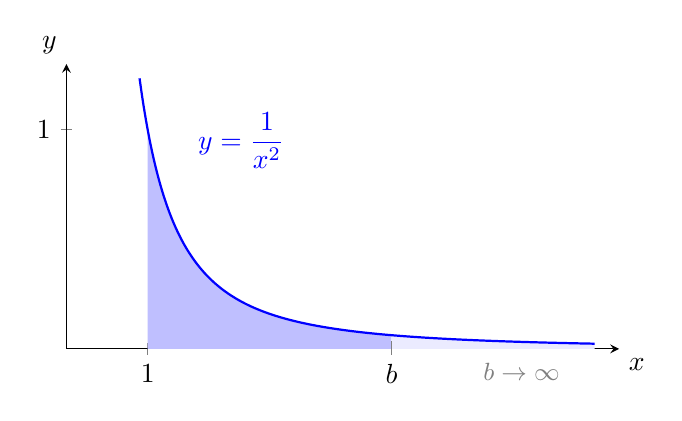
\begin{tikzpicture}
	\begin{axis}[
		axis lines=middle,
		xmin=0, xmax=6.8,
		ymin=0, ymax=1.3,
		xtick={1,4}, xticklabels={$1$,$b$}, ytick={1},
		xlabel={$x$}, ylabel={$y$},
		xlabel style={below right}, ylabel style={above left},
		samples=200, smooth, clip=false,
		width=8.6cm, height=5.2cm
		]
		\addplot[name path=f, thick, blue, domain=0.9:6.5] {1/x^2};
		\addplot[name path=ax, draw=none, domain=0.9:6.5] {0};
		\addplot[blue!25] fill between[of=f and ax, soft clip={domain=1:4}];
		\addplot[blue!8] fill between[of=f and ax, soft clip={domain=4:6.5}];
		\draw[dashed, gray] (axis cs:4,0) -- (axis cs:4,0.0625);
		\node[blue, anchor=west] at (axis cs:1.5,0.95) {$y=\dfrac1{x^2}$};
		\node[gray, anchor=north, font=\small] at (axis cs:5.6,-0.02) {$b\to\infty$};
	\end{axis}
\end{tikzpicture}
\end{document}
